\documentclass{article}

\usepackage{fancyhdr}
\usepackage{hyperref}
\usepackage{titlesec}
\usepackage{graphicx}
\usepackage{tikz}
\usepackage{listings}
\usepackage{xcolor}
\usepackage[font=itshape]{quoting}
\definecolor{codegreen}{rgb}{0,0.6,0}
\definecolor{codegray}{rgb}{0.5,0.5,0.5}
\definecolor{codepurple}{rgb}{0.58,0,0.82}
\definecolor{backcolour}{rgb}{0.95,0.95,0.92}


\lstdefinestyle{mystyle}{
    backgroundcolor=\color{backcolour},   
    commentstyle=\color{codegreen},
    keywordstyle=\color{magenta},
    numberstyle=\tiny\color{codegray},
    stringstyle=\color{codepurple},
    basicstyle=\ttfamily\footnotesize,
    breakatwhitespace=false,         
    breaklines=true,                 
    captionpos=b,                    
    keepspaces=true,                 
    numbers=left,                    
    numbersep=5pt,                  
    showspaces=false,                
    showstringspaces=false,
    showtabs=false,                  
    tabsize=2
}

\lstdefinelanguage{JavaScript}{
  keywords={typeof, new, true, false, catch, function, return, null, catch, switch, var, if, in, while, do, else, case, break},
  keywordstyle=\color{blue}\bfseries,
  ndkeywords={class, export, boolean, throw, implements, import, this},
  ndkeywordstyle=\color{darkgray}\bfseries,
  identifierstyle=\color{black},
  sensitive=false,
  comment=[l]{//},
  morecomment=[s]{/*}{*/},
  commentstyle=\color{purple}\ttfamily,
  stringstyle=\color{red}\ttfamily,
  morestring=[b]',
  morestring=[b]"
}

\lstset{style=mystyle}

\usetikzlibrary{shapes,arrows}
\newcommand{\comment}[1]{}


\tikzstyle{decision} = [diamond, draw, 
    text width=4.5em, text badly centered, node distance=3cm, inner sep=0pt]
\tikzstyle{line} = [draw, -latex']
\tikzstyle{block} = [rectangle, draw, 
    text width=8em, text centered, rounded corners, minimum height=4em]
\tikzstyle{start} = [rectangle, draw, 
    text width=4.5em, text badly centered, rounded corners, node distance=3cm]
\tikzstyle{io} = [trapezium, trapezium left angle=70, trapezium right angle=110, minimum width=3cm, minimum height=1cm, text centered, draw=black]


\setcounter{secnumdepth}{5}
\setcounter{tocdepth}{4}

\pagestyle{fancy}
\fancyhf{}
\rhead{Path-finding Algorithms and Solving Mazes}
\lhead{Oliver Temple [CN]}
\rfoot{\thepage}
\lfoot{Path-finding Algorithms and Solving Mazes}

\title{Path-finding Algorithms and Solving Mazes}

\author{Oliver Temple}

\begin{document}

\maketitle
\tableofcontents

\section{analysis}
\subsection{Project Description}
Path finding algorithms are essential in many aspects of computer science, from computer games to solving complex real world problems, however they can be complex things to visualize, especially when learning about them for the first time. This project's aim to create a path finding visualization tool that will generate and solve mazes, and to provide a general understanding of the algorithms used. 

There are a number of different algorithms that can be used to solve and generate mazes, and this project will focus on the more common ones like Dijkstra's, Depth First Search, Prims and more. I intend to include algorithms that are different from each other to show the advantages and disadvantages of each.

\subsection{Research}
\subsubsection{Overview}
To complete this project, I will need a strong understanding of maze generation and path finding algorithms, how they work and how to model them, knowledge of react and javascript to create a website for the visualization as well as user opinions on what features are needed.
\subsubsection{Research Log}
I was introduced to path finding algorithms in one of my lessons, where we learned what they were used for and some examples, as well as how they can be modeled. For example, modelling the maze as a graph with weighted nodes of 1 and 0, for the walls and space respectively. The algorithms we looked at were Dijkstra's and A*. We also looked at Prim's algorithm, recursive backtracking, depth fist search and Kruskal's algorithms for maze generation.

\paragraph{Maze Generating Algorithms}
\subparagraph*{Prims}
In class, we were taught about Prim's algorithm, and how it works. I used the information that our teacher gave us to write my own implementation of Prim's algorithm.
\subparagraph*{Recursive Backtracking}
When researching recursive backtracking I can across a website that said:
\begin{quoting}
    Here's the mile-high view of recursive backtracking:
    \begin{enumerate}
        \item Choose a starting point in the field.
        \item Randomly choose a wall at that point and carve a passage through to the adjacent cell, but only if the adjacent cell has not been visited yet. This becomes the new current cell.
        \item If all adjacent cells have been visited, back up to the last cell that has uncarved walls and repeat.
        \item The algorithm ends when the process has backed all they way up to the starting point. 
    \end{enumerate}
\end{quoting}
\url{https://weblog.jamisbuck.org/2010/12/27/maze-generation-recursive-backtracking}
I used this along with another visualization that I found to write my own recursive backtracking algorithm.

\paragraph{Path Finding Algorithms}
\subparagraph*{Depth First Search}
For the depth first search, I looked \url{https://isaaccomputerscience.org/concepts/dsa_pathfinding_dfs_bfs?examBoard=ocr&stage=a_level}, a resource I often use for studying. I used their easy to understand description to write my own implementation of depth first search. Their website said:
\begin{quoting}
    A depth-first search begins at the start node and then searches as far as possible down a branch of the graph, moving forward until there are no more nodes along the current branch to be explored. If the target node is found along the way, the search can stop. Otherwise, it must backtrack and find another branch to explore.

    This process uses a stack as a supporting data structure to keep track of the nodes that have not been fully explored. As each node is discovered, it is added to the stack.
\end{quoting}

\subparagraph*{Breadth First Search}
Isaaccomputerscience also have a page on breadth first search, also containing a simple description that I used to implement my own breadth first search.
\begin{quoting}
    The algorithm starts searching at a designated start node and searches through all the adjacent nodes (neighbours) before moving on. You can think of this process as moving out in waves from a given point. Another simple way to visualise a breadth-first search algorithm is to imagine that you are making a cake one layer at a time. You can't add the next layer unless the previous one is complete.

    This process uses a queue as a supporting data structure to keep track of the nodes that have not been fully explored. As each node is discovered, it is added to the queue.
\end{quoting} 

\subparagraph*{Dijkstra's}
For dijkstr's, i found this website:\url{https://daemianmack.org/posts/2019/12/mazes-for-programmers-dijkstras-algorithm.html}, that had a very good description of Dijkstra's algorithm. 
\begin{quoting}
    \begin{enumerate}
        \item Determine the starting point of the grid.
        \item Record the cost of reaching that cell: 0.
        \item Find that cell's navigable neighbors.
        \item For each neighbor, record the cost of reaching that neighbor: 1.
        \item For each neighbor, repeat steps 3-5, taking care not to revisit already-visited cells.
    \end{enumerate}
\end{quoting}

\subparagraph*{Greedy Search}
Having researched the other path finding algorithms, and learnt about greedy algorithms in class, I used the knowledge I already had to write my own greedy search algorithm.

\subsection{Project Background}
\subsubsection{Current Systems}
\paragraph{Example 1}
\href{https://clementmihailescu.github.io/Pathfinding-Visualizer/
}{https://clementmihailescu.github.io/Pathfinding-Visualizer
}
\newline
In this example, mazes can be generated with various algorithms, as well as being drawn by the user. The mazes can also be edited after they have been generated. The available maze generation algorithms are:
\begin{itemize}
    \item Recursive Division
    \item Recursive Division (vertical skew)
    \item Recursive Division (horizontal skew)
    \item Basic Random Maze
    \item Basic Weight Maze
    \item Simple Stair Pattern
\end{itemize}
These mazes can then be solved with a number of different path finding algorithms. The available path finding algorithms are:
\begin{itemize}
    \item Djikstra's Algorithm
    \item A* Search
    \item Greedy Best-first Search
    \item Swarm Algorithm
    \item Convergent Swarm Algorithm
    \item Bidirectional Swarm Algorithm
    \item Breadth-first Search
    \item Depth-first Search
\end{itemize}
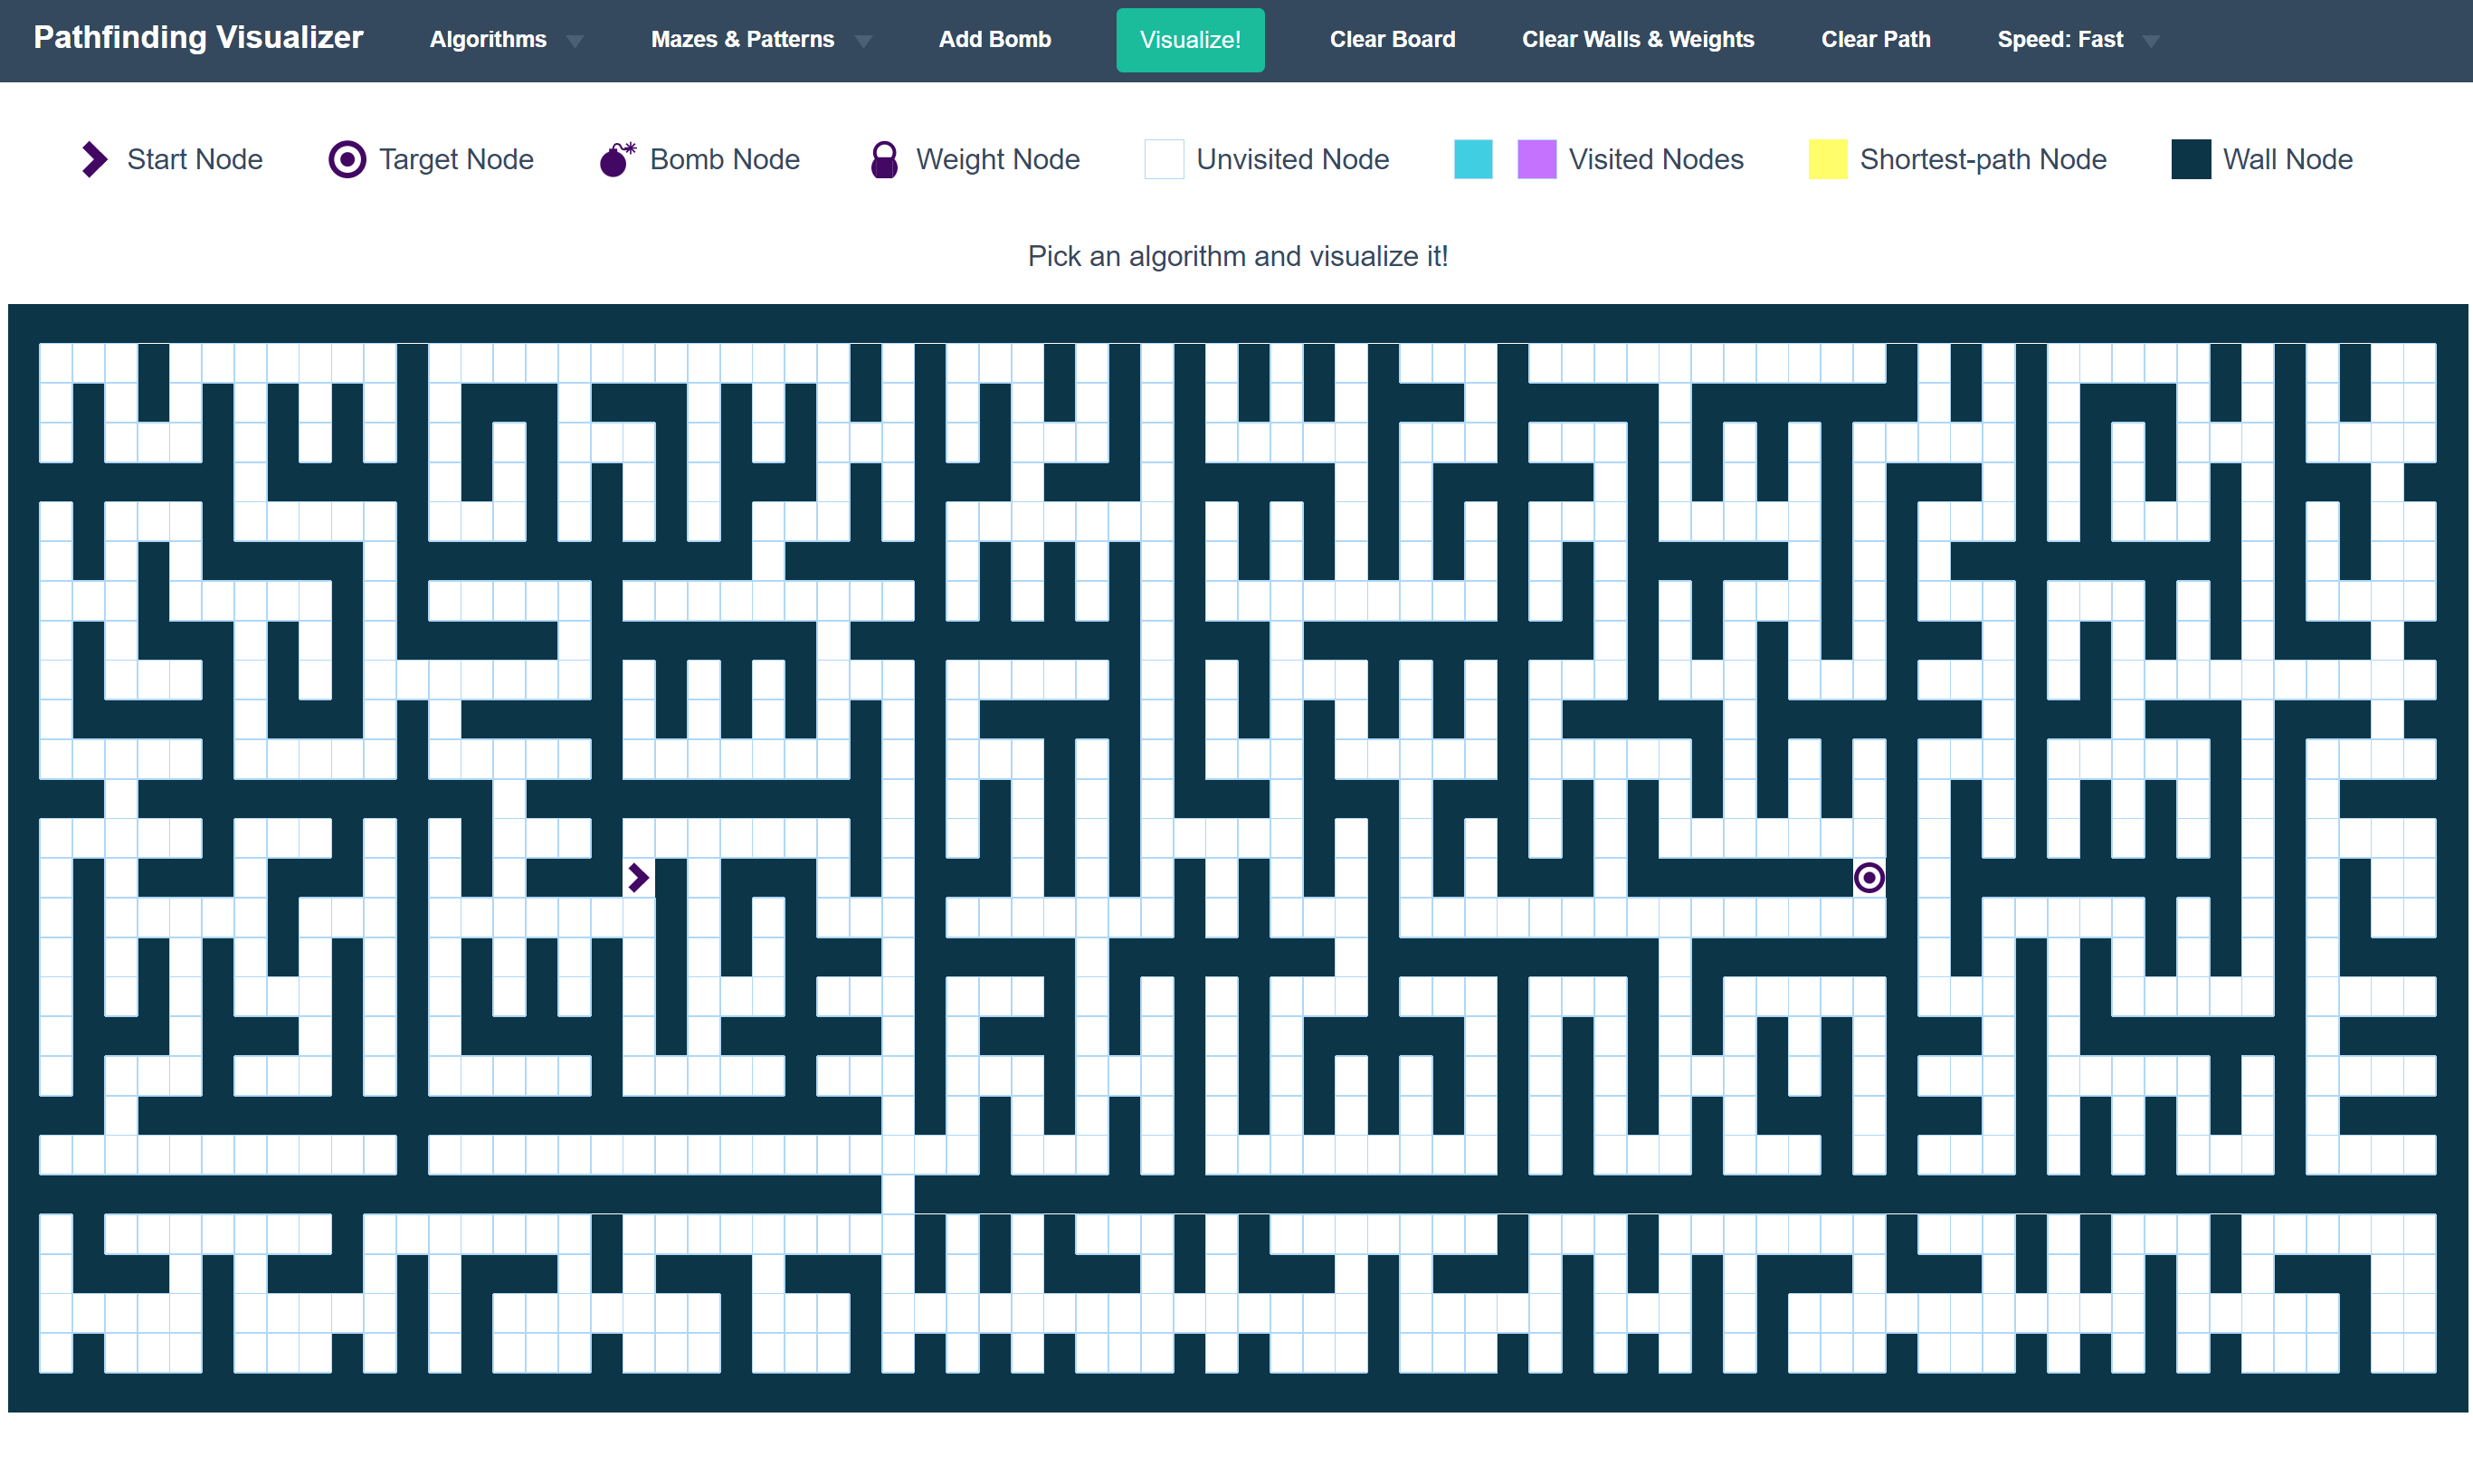
\includegraphics[width=\linewidth]{assets/Existing Solutions/example 1.PNG}
\subparagraph*{pros}
\begin{itemize}
    \item Many different algorithms to choose from.
    \item Start and end nodes can be moved.
    \item Maze can be altered.
    \item If nodes are moved after visualization has run, then the visualization will update.
    \item "Bomb" node, adds a via point that the path must go through.
\end{itemize}
\subparagraph*{cons}
\begin{itemize}
    \item The visualization is too slow.
    \item If maze is altered by user after visualization has run, then the visualization will not update.
\end{itemize}


\paragraph{Example 2}
\href{https://qiao.github.io/PathFinding.js/visual/
}{https://qiao.github.io/PathFinding.js/visual/
}
\newline
In this example, mazes have to be drawn by the user. The maze can then be solved with a number of different algorithms, however, these algorithms have more choice. For example, in the A* option, you can change the heuristic that is used. The available algorithms are:
\begin{itemize}
    \item A*
    \item IDA*
    \item Breadth-First-Search
    \item Best-First-Search
    \item Dijkstra
    \item Jump Point Search
    \item Orthogonal Jump Point Search
    \item Trace
\end{itemize}
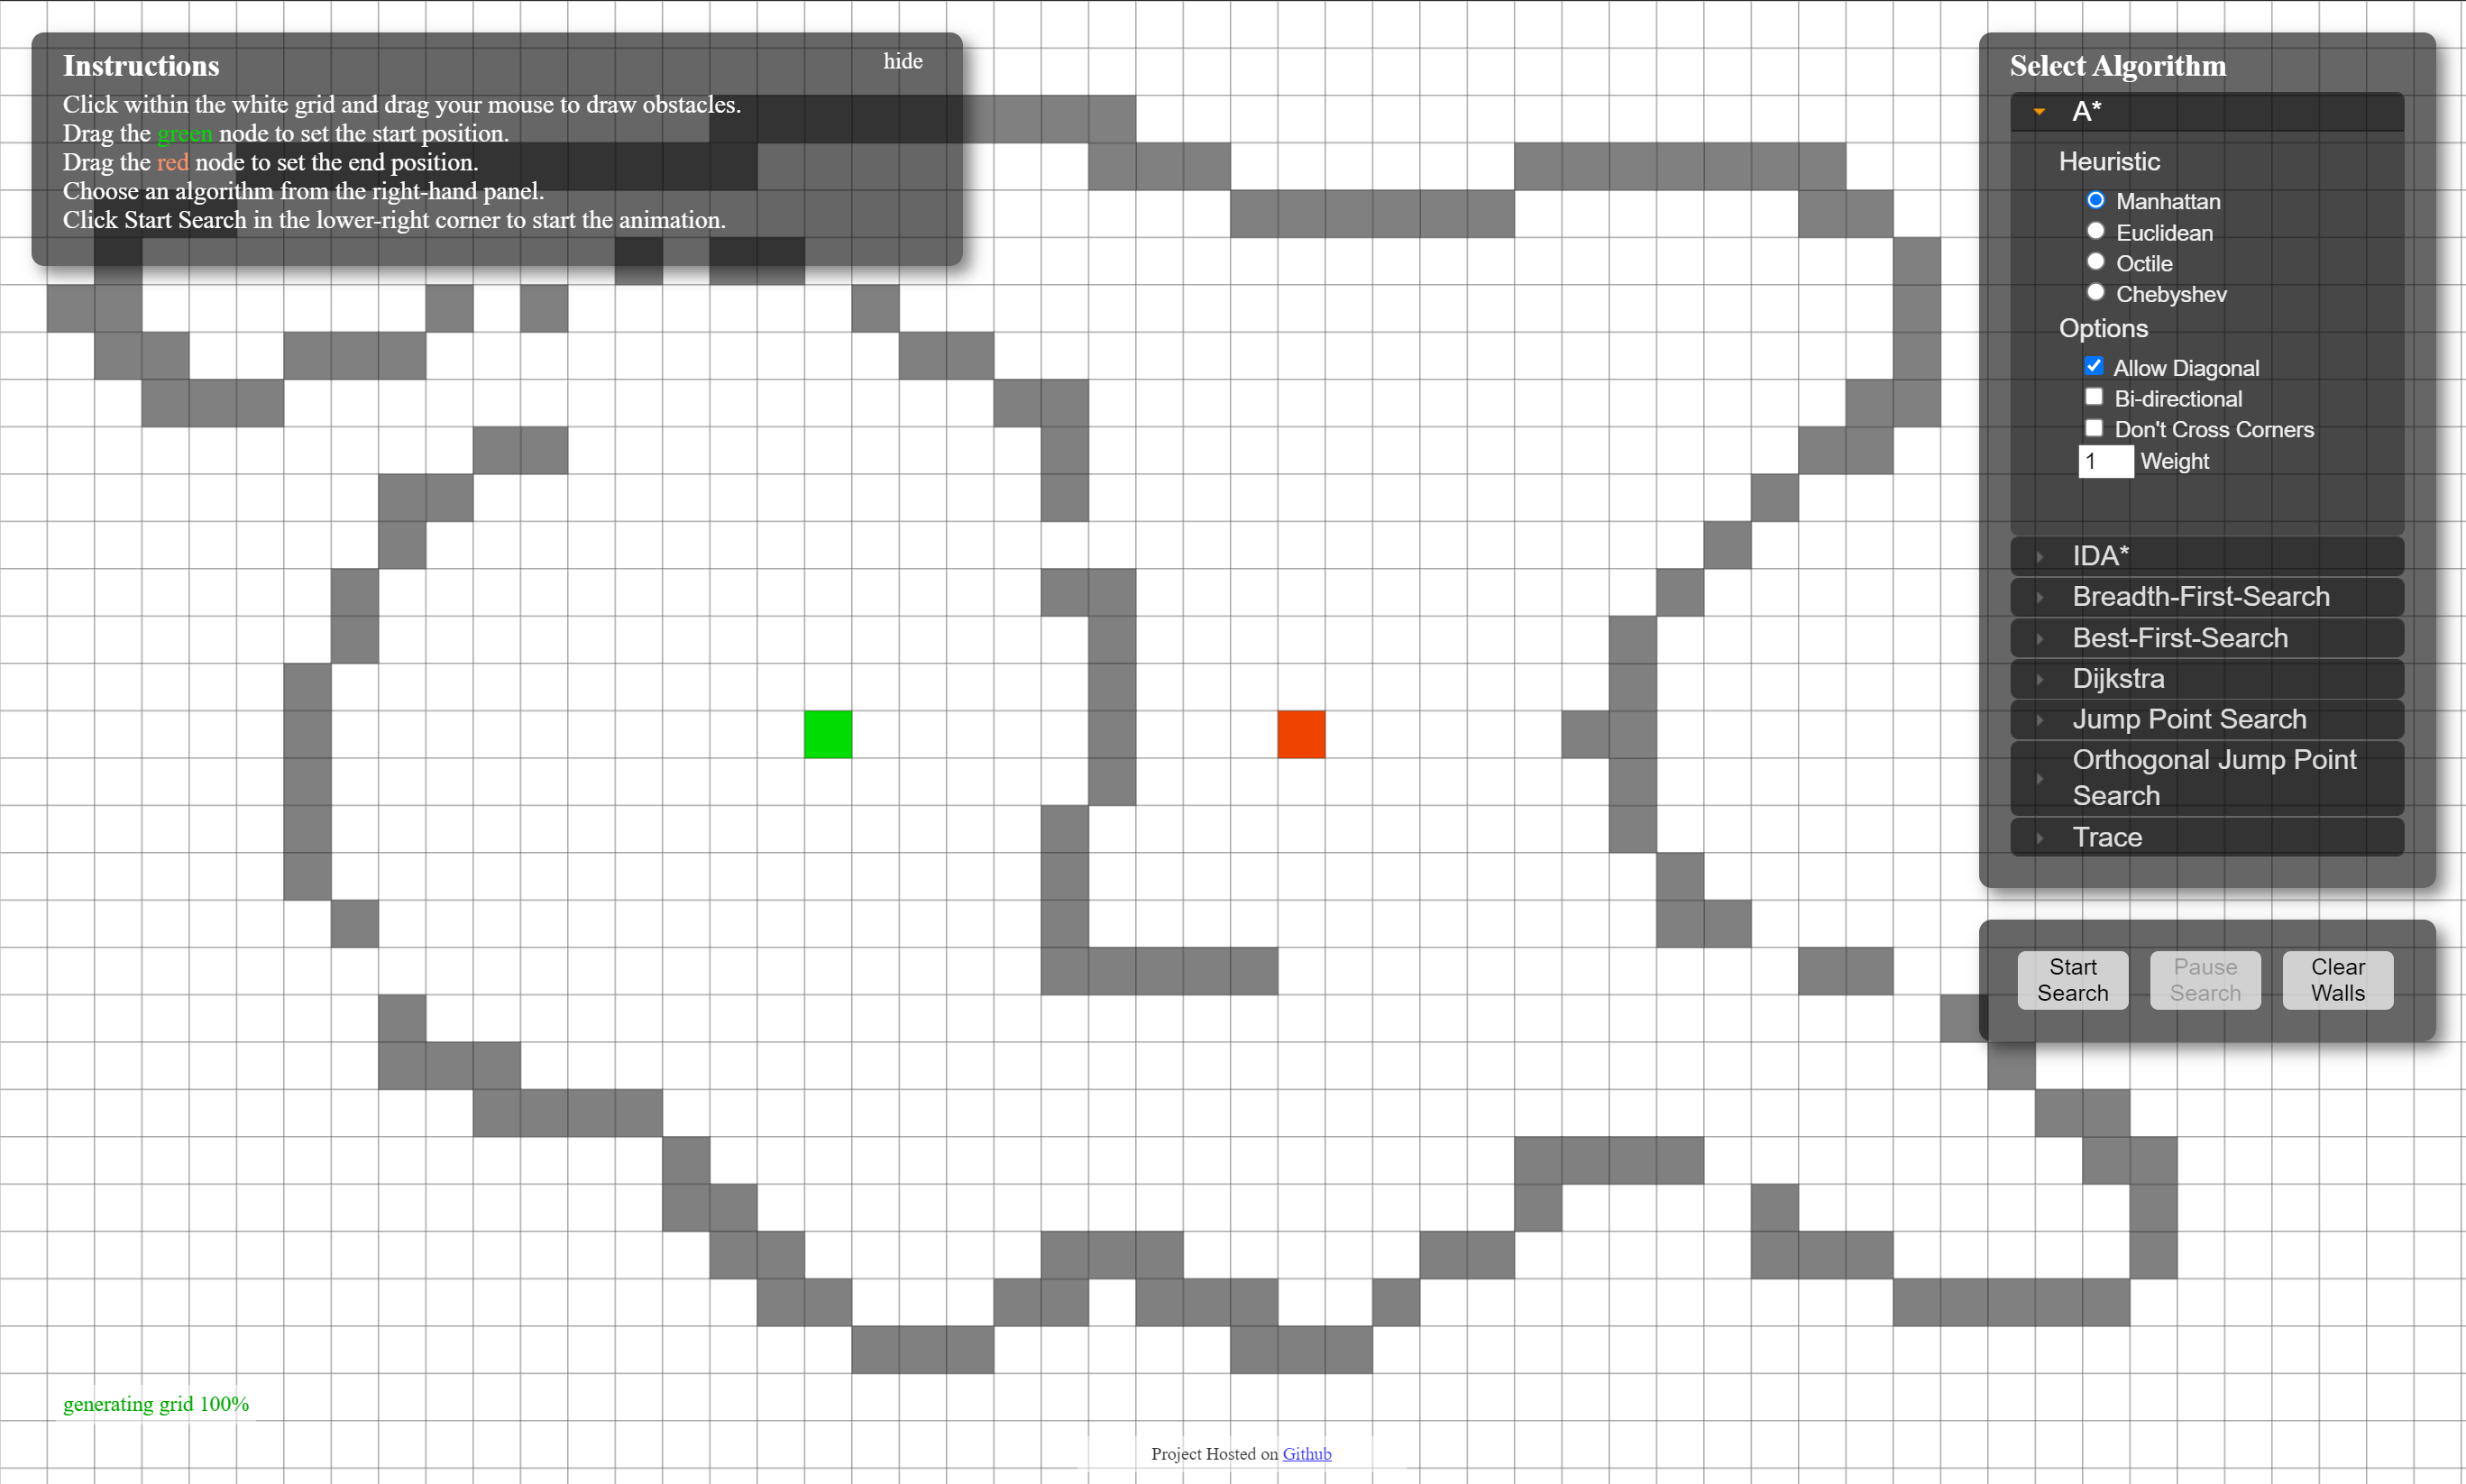
\includegraphics[width=\linewidth]{assets/Existing Solutions/example 2.PNG}
\subparagraph*{pros}
\begin{itemize}
    \item More options to choose from within each algorithm.
\end{itemize}
\subparagraph*{cons}
\begin{itemize}
    \item No maze generation.
    \item Visualization does not update when maze or start/finnish nodes are changed.
\end{itemize}


\paragraph{Example 3}
\href{https://pathfindout.com/
}{https://pathfindout.com/
}
\newline
In this example, mazes can be generated or drawn, however, mazes can only be generated with the recursive division algorithm. There are fewer path finding algorithms to solve the mazes than the others. The available algorithms are:
\begin{itemize}
    \item Dijkstra's Algorithm
    \item A* Search
    \item Breadth First Search
    \item Depth First Search
\end{itemize}
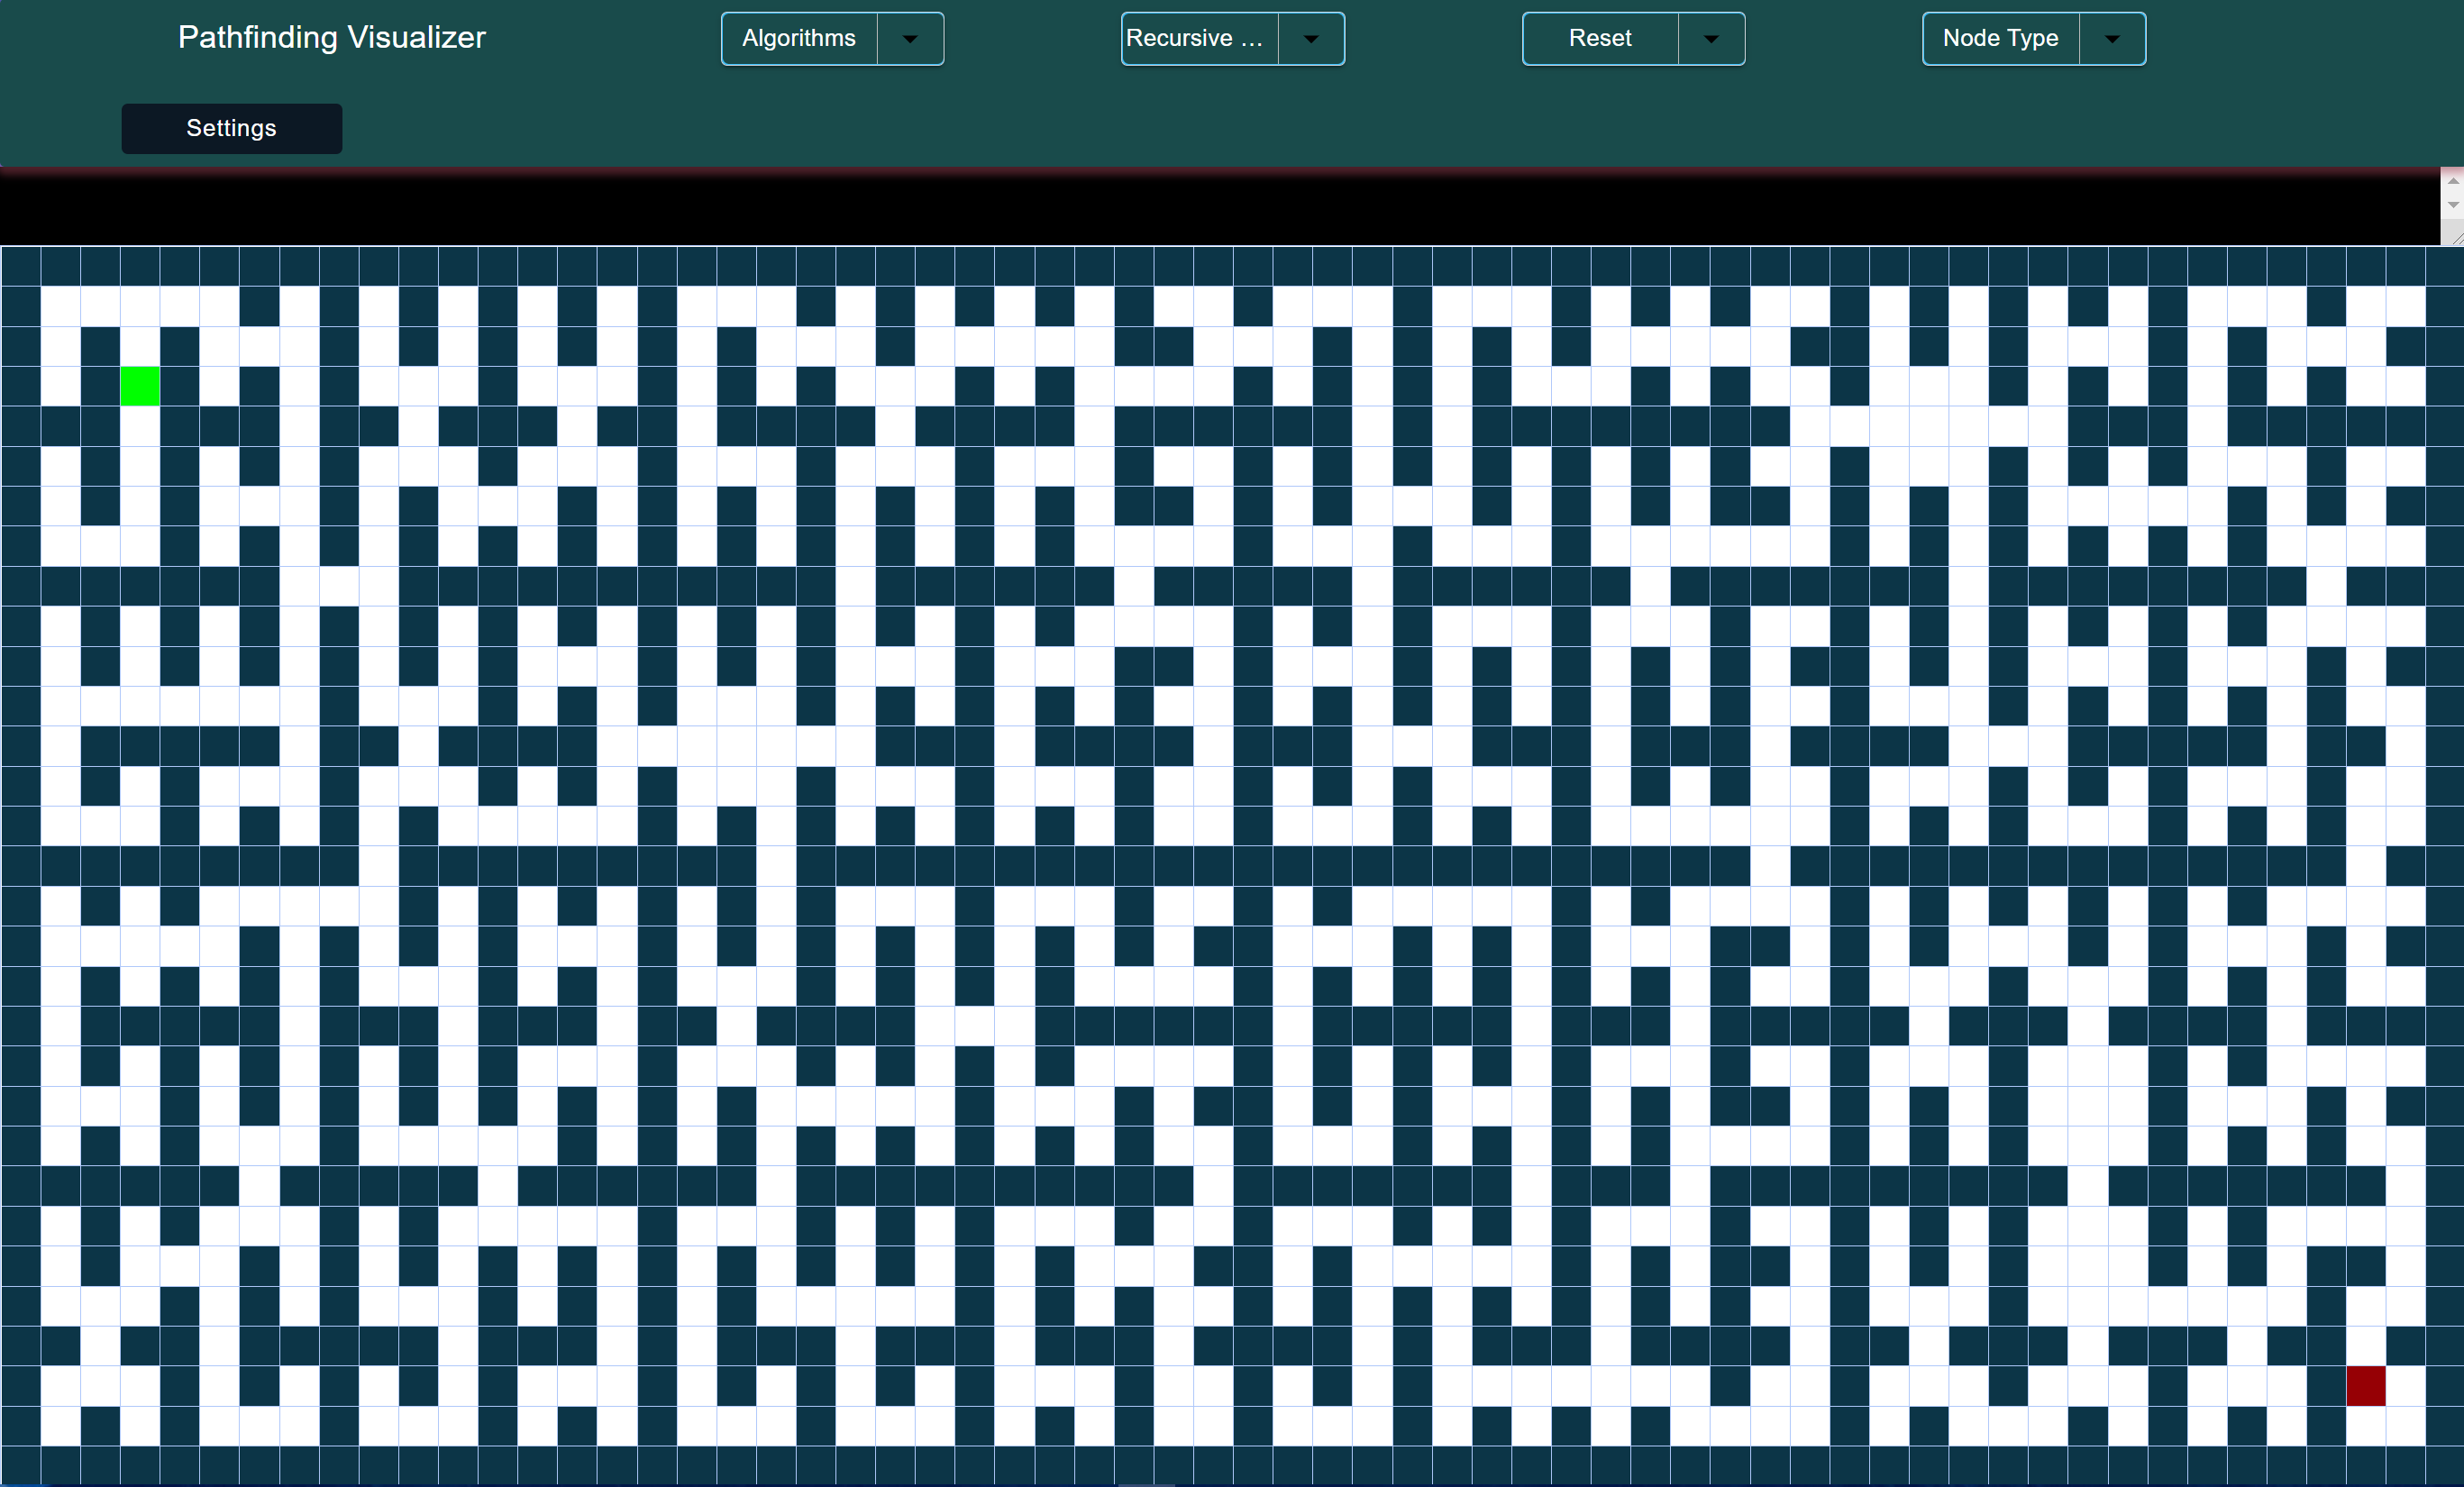
\includegraphics[width=\linewidth]{assets/Existing Solutions/example 3.PNG}
\subparagraph*{pros}
\begin{itemize}
    \item Different weighted nodes available.
    \item Shows how many nodes visited.
    \item Shows final path length.
    \item Data structure for some algorithms can be changed.
    \item Weights of specific node types can be changed.
    \item Node size can be changed.
\end{itemize}
\subparagraph*{cons}
\begin{itemize}
    \item Sometimes generates mazes that cannot be solved.
    \item Cannot edit maze after visualization has run.
    \item Only one maze generation algorithm.
    \item Fewer path finding algorithms to solve the maze.
\end{itemize}

\subsubsection{Proposed Solution}
I will make a path-finding visualization that encompasses as many of the merits of the existing solutions as possible, while also tackling as many of the drawbacks.
\begin{itemize}
    \item Research the different algorithms needed and write the corresponding pseudoscode.
    \item Create a mockup of the user interface.
    \item Create the user interface in react.
    \item Code the algorithms in python.
    \item Create an AWS lambda function in python that runs the algorithms as an API.
    \item Create the react website to visualize the algorithms.
    \item Add additional features suggested by end users.
    \item Test visualization and check that it meets all of the objectives.
\end{itemize}
\subsubsection{Prospective Users}
The users of this system will most likely consist of teachers and students who are learning about path finding algorithms as it will clearly show how the algorithms function.
\paragraph{Questions To Users}
I asked some prospective users some questions about what they would like to see in the visualizer.
\paragraph*{Questions}
\begin{enumerate}
    \item[Q1.]What algorithms would you like to see for maze generation?
    \item[Q2.]What algorithms would you like to see for solving the maze?
    \item[Q3.]What additional features would you like to see in the path finding visualization?
    \item[Q4.]Would it be useful to be able to write your own path finding algorithms that can be run in the visualization?  
\end{enumerate}
\paragraph*{Answers}
\begin{enumerate}
    \item[A1.]I would like to see recursive backtracking and Prim's algorithms used for maze generation, as well as Kruskal's (less important). This is because Kruskal's and Prims are similar but each has their own advantages and disadvantages and recursive backtracking is different and uses recursion.
    \item[A2.]I would like to see an algorithm(such as Dijkstra's) as well as a heuristic(such as A* or a greedy search), as this will show the difference between a heuristic and an algorithm.
    \item[A3.]Option to add your own png image for the drawing of final path - "a sussy imposter running around the maze".
    \item[A4.]I would find it useful to be able to code my own algorithms. This would allow me to use the visualization with other, lesser known algorithms that I may want to visualize.
\end{enumerate}
The answers to these questions confirms what is required from the visualization, which will be reflected in the objectives. The need for contrasting algorithms is something that I will consider when deciding what algorithms to use.
\subsection{Objectives}
\subsubsection{Generate Mazes}
The website should be able to generate mazes using multiple algorithms, including, but not limited to: Prim's algorithm and recursive backtracking. There should also be a brief description of the algorithm that has been selected.

\subsubsection{Solve Mazes}
The website should be able to solve mazes using multiple algorithms, including, but not limited to: greedy search, Dijkstra's algorithms, depth-first search and breadth-first search. There should also be a brief description of the algorithm that has been selected.

\subsubsection{Customisation}
The user should be able to customize aspects of the visualization, including:
\begin{itemize}
    \item Size of the maze.
    \item Speed of the animation.
    \item The heuristic used in any heuristic algorithms.
\end{itemize}

\subsubsection{User written algorithms}
The website should be able to run algorithms written by the user for both maze generation and solving. This will be done by supplying documentation on what parameters need to be taken in and what will need to be returned from the function for the visualizer to work.

\subsubsection{Update Visualization}
If the start or end nodes are moved once the visualization has been run, then it should update without the user having to rerun the visualization.

\subsubsection{Special Nodes}
There should be "special" nodes that are different from walls or space. For example, nodes with different weights or a "via point" node that the path must go through.

\section{Documented Design}
\subsection{Visualization Structure}

There will be a python API for generating and solving the mazes, and a react website that will visualize the algorithms. There will be one API endpoint, however different parameters will be passed to determine weather the api should solve or generate, and which algorithms to use. These parameters will be:
\begin{itemize}
    \item width
    \item height
    \item type (solve/generate/empty maze)
    \item generate (algorithm for generation)
    \item solve (algorithm for solving)
    \item start
    \item end
\end{itemize} 

When solving the maze, the maze will be sent to the API as part of the body of the request.
\newline
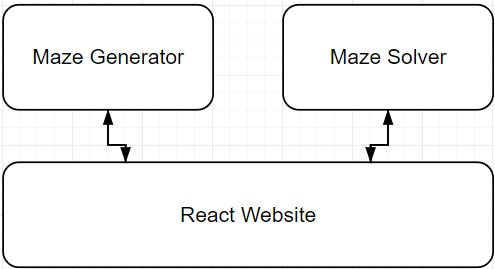
\includegraphics[width=\linewidth]{assets/structure.jpg}
\subsection{Flow Chart}
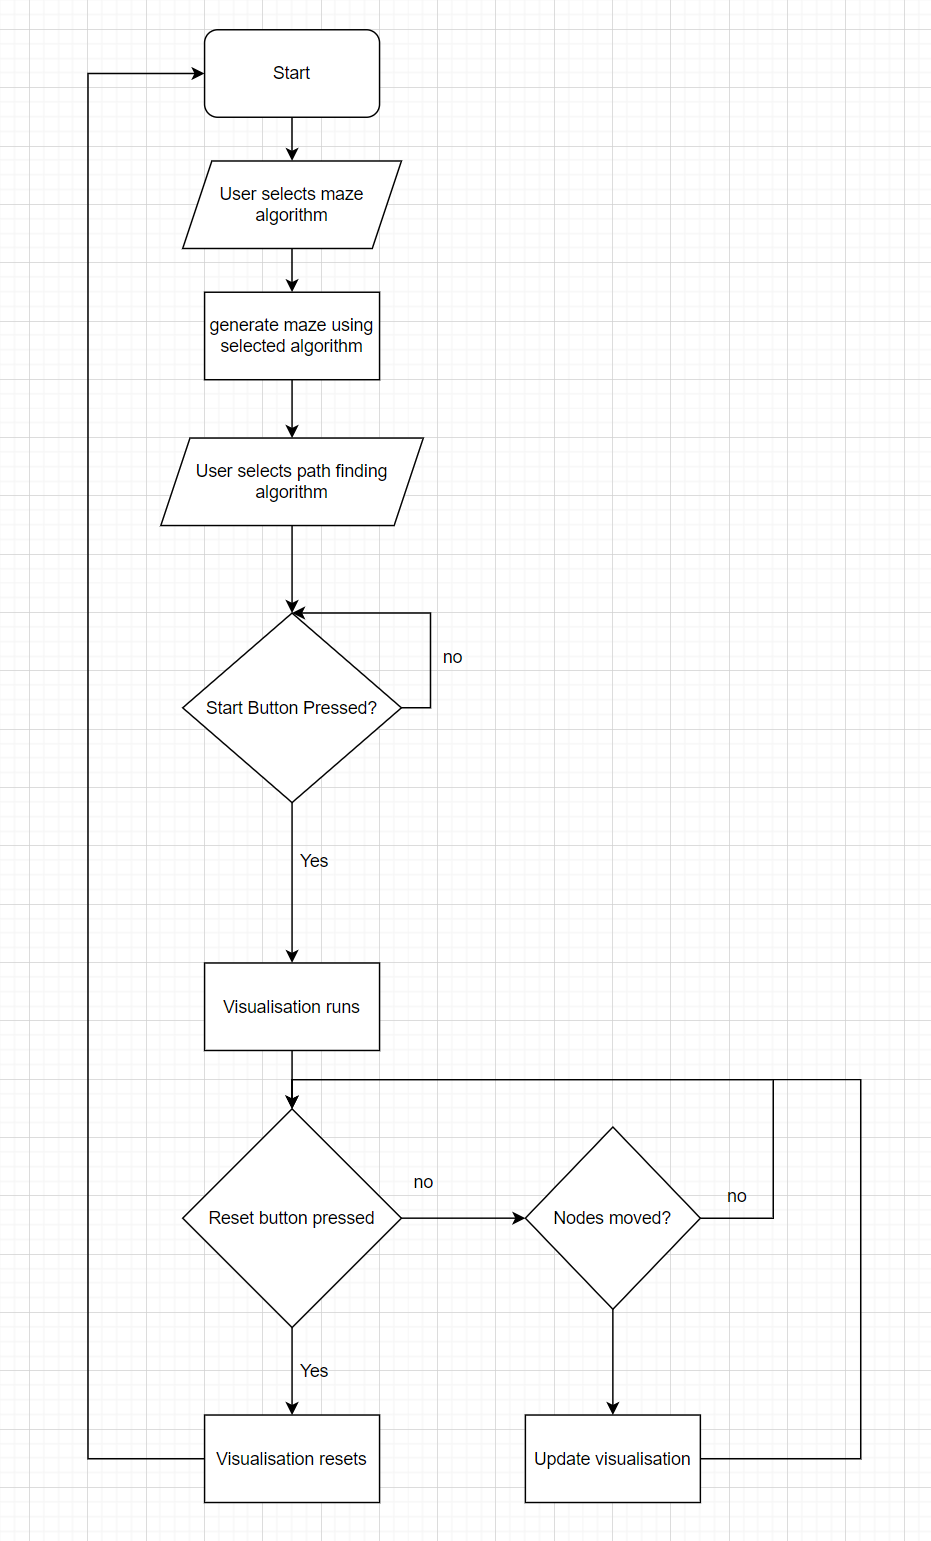
\includegraphics[width=\linewidth, height=17.5cm]{assets/flow chart.PNG}

\subsection{User Interface}
I have used Figma to create a design mockup of how the user interface will look. This allows me to plan what user inputs will be needed.
\newline
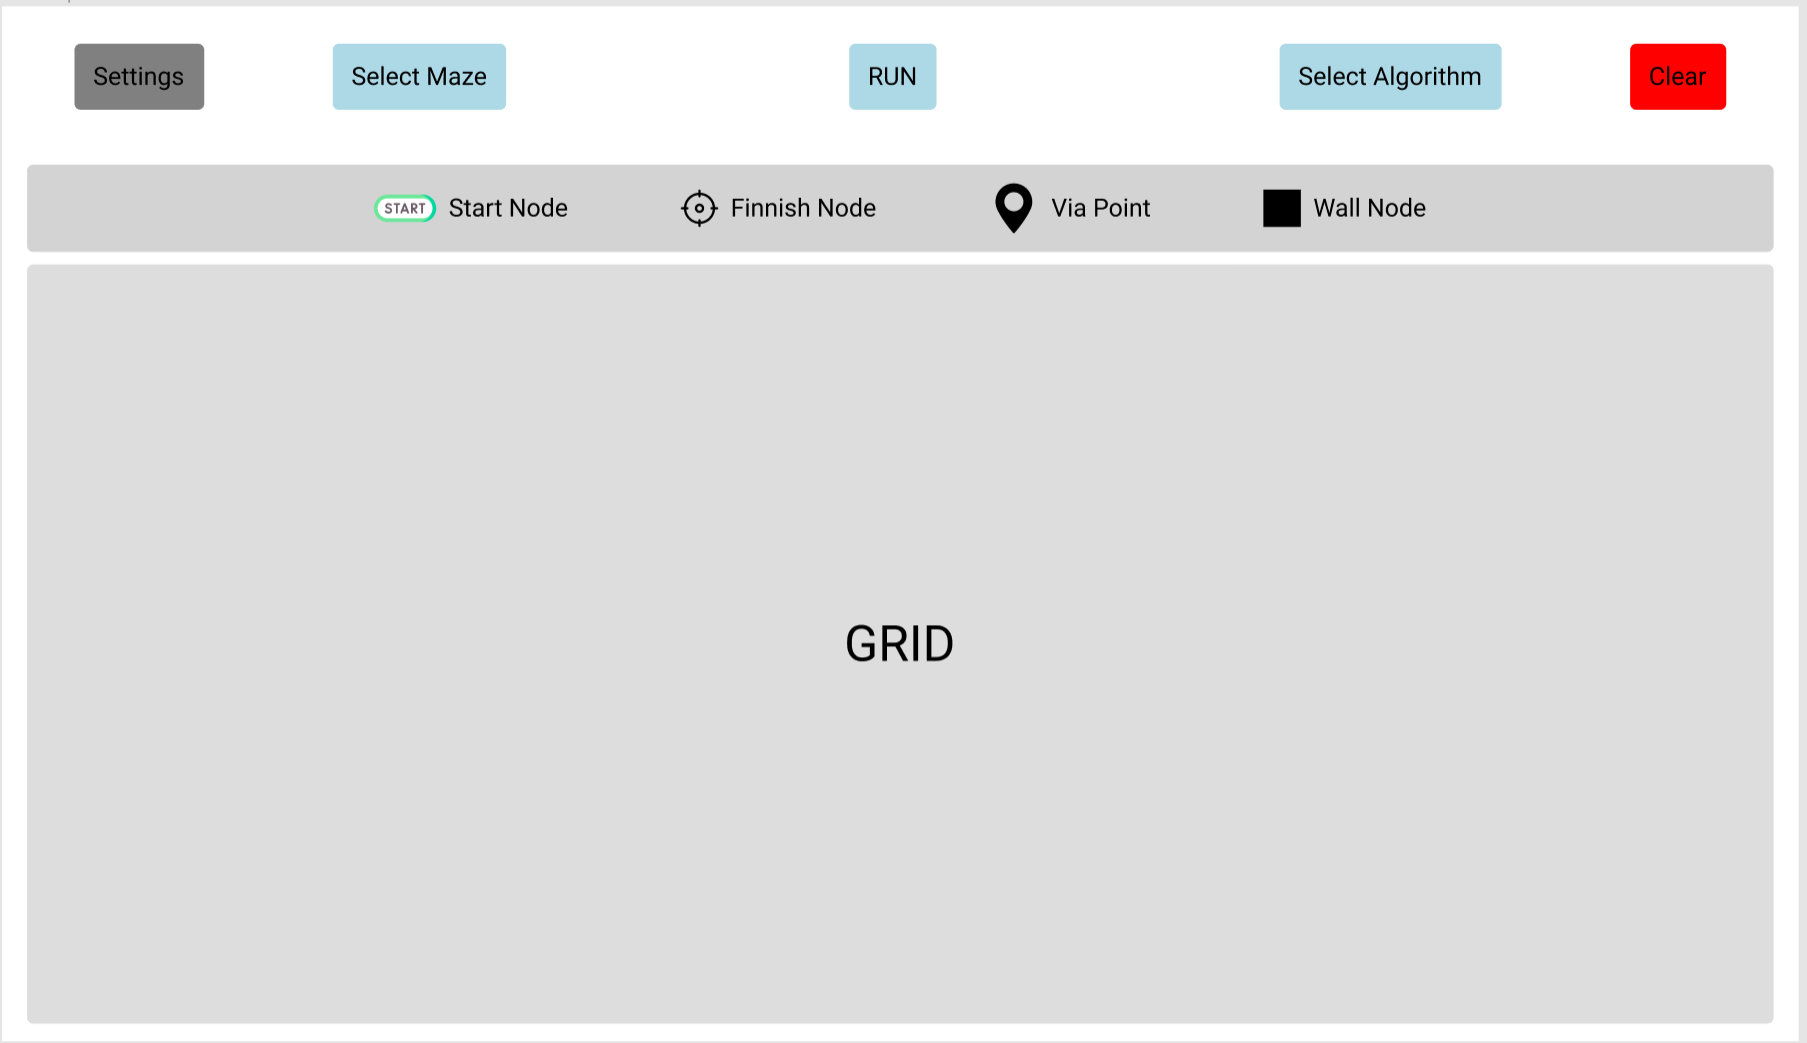
\includegraphics[width=\linewidth]{assets/gui.PNG}
\subsection{Class Diagrams}
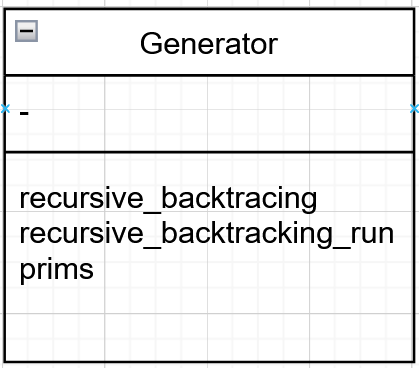
\includegraphics[width=0.5\linewidth]{assets/class diagrams/generator.PNG}
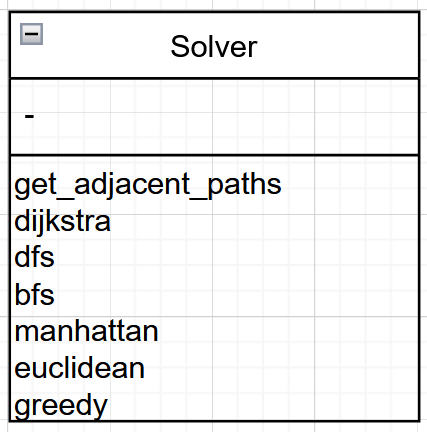
\includegraphics[width=0.5\linewidth]{assets/class diagrams/solver.PNG}
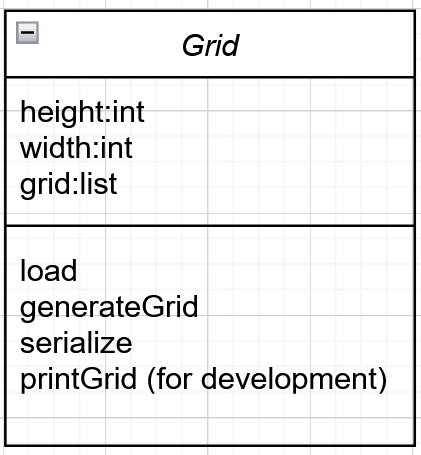
\includegraphics[width=0.5\linewidth]{assets/class diagrams/maze.PNG}
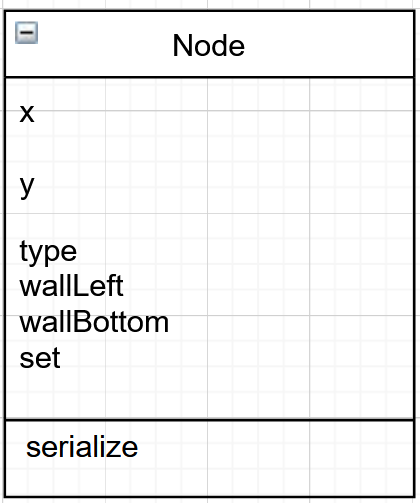
\includegraphics[width=0.5\linewidth]{assets/class diagrams/node.PNG}

\subsection{Algorithms}
\subsubsection{Prims}
Prim's algorithm will have two lists, an inMaze list and a frontier, to store the nodes that are in the maze and in the frontier respectively. To start, the nodes adjacent to the start node will be added to the frontier. Then a random wall will be taken from the frontier, and the wall will be removed from the maze. The node that was connected by removing the wall will then be added to the inMaze list. Any nodes that are adjacent to the new node and not in the maze will be added to the frontier. This will continue while there are nodes in the frontier.

\subsubsection{Recursive Backtracking}
Recursive backtracking will use a stack to store the previous nodes that have been visited. The stack will be a list of Nodes that are added to the stack as they are visited. If the algorithm reaches a node that has no unvisited adjacent nodes, then the algorithm will backtrack to the last node that was visited by popping off of the stack. This will continue until the algorithm backtracks to the start node.

\subsubsection{Dijkstra's}
Dijkstra's algorithm works by keeping a priority queue of the nodes that have not been visited, however, all connections have the same weights, as it is solving a maze. The queue will be a list of Nodes, with their distance initially set to "infinity". The algorithm will then search outwards from the start node, adding the distance from the start to each node as it is discovered, until the end node is reached. The algorithm will then backtrack from the end node to the start node, choosing the node with the lowest distance at each step.

\subsubsection{Depth First Search}
Depth first search(dfs) works by keeping a stack of the nodes that need to be visited, and adding to the stack as new nodes are discovered. When the nodes are added to the stack, the "parent" attribute of the nodes will be updated so that a path can be drawn. If there are no unvisited nodes connected to the current node, then the algorithm will backtrack by popping a node off of the stack. This will continue until the stack is empty or the end node is reached, at which point the algorithm will return and a path will be drawn.

\subsubsection{Breadth First Search}
Breadth first search(bfs) is similar to dfs, however a queue should be used instead of a stack. The queue will be a list of Nodes, with new Nodes being added to the end of the list as they are discovered. When the nodes are added to the queue, the "parent" attribute of the nodes will be updated so that a path can be drawn. The algorithm will keep searching until the queue is empty or the end node is reached, at which point the algorithm will return and a path will be drawn.

\subsubsection{Greedy Search}
Greedy search works by keeping a priority queue, with the heuristic distance from the node to the end node being the priority. The algorithm will start from the start node, searching outwards, adding nodes to the priority queue as they are discovered, with the "parent" attribute being updated so that the path can be drawn. The algorithm will keep searching until the queue is empty or the end node is reached, at which point the algorithm will return and a path will be drawn.
\paragraph*{Heuristic}
Different heuristics can be used for the greedy search. The heuristic I will include are manhattan distance and euclidean distance, as these are some of the most common heuristics.

\subparagraph*{Manhattan Distance}
Manhattan is calculated by
\begin{equation}
    h(n) = |x_{current\ node} - x_{end\ node}| + |y_{current\ node} - y_{end\ node}|
\end{equation}
\subparagraph*{Euclidean Distance}
Euclidean is calculated by
\begin{equation}
    h(n) = \sqrt{(x_{current\ node} - x_{end\ node})^2 + (y_{current\ node} - y_{end\ node})^2}
\end{equation}
\comment{
\subsection{Algorithms}
\subsubsection{Maze generating algorithms}
Pseudoscode for the maze generation algorithms.
\paragraph{prims}
\begin{verbatim}
    function prims(Grid)
        let inMaze = [[0,0]]
        let frontier = [
            [[0,1],["left"]],
            [[1,0],["top"]]
        ]
        
        while frontier.length > 0
            new <- frontier.pop(rand(0, frontier.length - 1))
            toAdd <- new[0]
            wall <- new[1][rand(0, new[1].length - 1)]
            inMaze.push(toAdd)

            if wall == "bottom"
                Grid.grid[toAdd[0]][toAdd[1]].wallBottom = false
            if wall == "left"
                Grid.grid[toAdd[0]][toAdd[1]].wallLeft = false
            if wall == "top" and toAdd[0] > 0
                Grid.grid[toAdd[0] - 1][toAdd[1]].wallBottom = false
            if wall == "right" and toAdd[1] < Grid.width - 1
                Grid.grid[toAdd[0]][toAdd[1] + 1].wallLeft = false
            
            possible <- [
                [toAdd[0]-1, toAdd[1]],
                [toAdd[0]+1,toAdd[1]],
                [toAdd[0],toAdd[1]-1],
                [toAdd[0], toAdd[1]+1]
            ]

            walls <- ["bottom", "top", "right", "left"]

            for i in range 4
                p <- possible[i]
                wall <- walls[i]
                if p[0] >= 0 and p[0] < Grid.height and p[1] >= 0 and p[1] < Grid.width
                    if p not in inMaze
                        found <- false
                        for v in frontier
                            if v[0] == p
                                v[1].push(wall)
                                found = true
                        end for
                        if not found
                            frontier.push([p, [wall]])
            end for
        end while
    end function
\end{verbatim}
\paragraph{Recusive backtracking}
\begin{verbatim}
    function recursiveBacktracking(Grid)
        unvisited <- []
        for row in Grid.grid
            for items in row
                unvisited.push(items)
            end for
        end for

        start <- unvisited.pop(rand(0, unvisited.length - 1))
        recursive_backtracking_run(Grid, unvisited, start, [])
    end function

    function recursive_backtracking_run(Grid, unvisited, current, previous)
        orientation_options <- []
        if current.x > 0 and Grid.grid[current.y][current.x - 1] in unvisited
            orientation_options.push("left")
        end if

        if current.y > 0 and Grid.grid[current.y - 1][current.x] in unvisited
            orientation_options.push("top")
        end if

        if current.x < Grid.width - 1 and Grid.grid[current.y][current.x + 1] in unvisited
            orientation_options.push("right")
        end if

        if current.y < Grid.height - 1 and Grid.grid[current.y + 1][current.x] in unvisited
            orientation_options.push("bottom")
        end if

        if orientation_options.length > 0
            orientation <- orientation_options[rand(0, orientation_options.length - 1)]
            previous.push(current)

            if orientation == "left"
                connecting_cell <- Grid.grid[current.y][current.x - 1]
                cell.wallLeft = false
            
            else if orientation == "bottom"
                connecting_cell <- Grid.grid[current.y + 1][current.x]
                cell.wallBottom = false
            
            else if orientation == "right"
                connecting_cell <- Grid.grid[current.y][current.x + 1]
                connecting_cell.wallLeft = false
            
            else if orientation == "top"
                connecting_cell <- Grid.grid[current.y - 1][current.x]
                connecting_cell.wallBottom = false
            end if

            unvisited.remove(connecting_cell)

            recursive_backtracking_run(Grid, unvisited, connecting_cell, previous)
        else
            if previous.length > 0
                new <- previous.pop()
                recursive_backtracking_run(Grid, unvisited, new, previous)
            end if
        end if
    end function
\end{verbatim}
}
\section{Evidence of Completeness}  
%out of 15 marks, argument for why the project is complete. Which algorithms have been used?

\section{Technical Solution}
\lstinputlisting[language=python]{../python api/lambda_function.py}
\lstinputlisting[language=python]{../python api/generator.py}
\lstinputlisting[language=python]{../python api/grid.py}
\lstinputlisting[language=JavaScript]{../react app/src/App.js}
\lstinputlisting[language=JavaScript]{../react app/src/components/Menu.jsx}
\lstinputlisting[language=JavaScript]{../react app/src/components/MenuKey.jsx}
\lstinputlisting[language=JavaScript]{../react app/src/components/DisplayGrid.jsx}
\lstinputlisting[language=JavaScript]{../react app/src/components/DisplayNode.jsx}

\section{Testing}

\section{Evaluation}
\end{document}